
\subsection{A vector space of channels} % {{{
\cpnote{Falta lo de las clases de equivalencias, pero aun no encuentro el
espacio. Quizá cuando haga falta se puede poner}
% \janote{Pienso que sí porque puede y debería ser útil para la sección siguiente
% de generadores.}
\par
% Inversion de la relacion entre tau y p, y que las probablidiades deben ser positivas {{{

In this subsection we will provide a one-to-one relation between PCE quantum channels 
and the subspaces of a discrete vector subspace associated with the indices $\valpha$
labeling the components of a state; see \eref{eq:N_qubits_rho}.


Let us start by recalling that the problem of determining complete positivity
of a PCE can be recast as determining which vectors $\vtau$ are mapped via
$\san$
% \begin{equation}
% \san\vec\tau=2^N\vec p
% \label{eq:condition}
% \end{equation}
to a vector with positive entries $\lambda_\valpha$, as in \eref{eq:lambda:is:A:tau}. 
% \janote{Siento que hace falta un enunciado por aquí, al inicio de la sección, que haga
% que el lector se pueda colgar de la idea de los espacios vectoriales. Quizás algo 
% como}\janote{We will show how to associate unequivocally PCE quantum
% channels with vector spaces.}
% . In components, this would read 
% \begin{equation}
% % \left(
% \sum_\vbeta
% \san_{\valpha\vbeta} \,
% % \right)
% \tau_{\vec \beta}=2^Np_{\vec\alpha}
% \label{eq:A:tau:is:p}
% \end{equation}
% where
% $\san_{\vec\alpha\vec\beta} =\sa_{\alpha_1\beta_1}\cdot\ldots\cdot
% \sa_{\alpha_N\beta_N}$. 
Using the fact that $a^{-1}=a/4$, so 
% (so $A = A^{-1}/2^N$) 
\begin{equation}
A^{-1} = \frac{1}{4^N} A,
\end{equation}
we can directly invert \eref{eq:lambda:is:A:tau} to obtain 
\begin{equation}
% \tau_{\vec \alpha}= \san_{\vec\alpha\vec\beta} \, p_\vbeta,
% \tau = 
% \san \lambda =2^N \tau
\sum_\vbeta \san_{\valpha \vbeta} \lambda_\vbeta =2^N \tau_\valpha
\label{eq:tau:is:A:p}
\end{equation}
which will serve as a starting point for our analysis. 
This is a remarkable equation, as it provides a method to diagonalize the
Choi matrix of any diagonal 
Pauli channel, as in \eref{eq:definition:Pauli}. 
% \janote{por qué diagonalizar al 
% canal de Pauli? Creo que sería más bien a la matriz de Choi, pero igual estoy 
% un poco pérdido con el sentido del enunciado. }


Other two simple but crucial
observation are the following. For valid quantum channels, 
% \begin{equation}
% % \sum_{
% \end{equation}
$\sum_{\valpha \in \Omega} \lambda_\valpha=0$ implies that 
$\lambda_\valpha=0$ for all $\valpha$ in an arbitrary subset of 
multi-indices $\Omega$, as each member of the sum is
greater or equal to zero, 
% $p_{\vec\alpha}+p_{\vec\beta}=0$ implies $p_{\vec\alpha}=p_{\vec\beta}=0$, as
% all $p_{\vec\alpha} \ge 0$
due to complete positivity of the underlying channel. 
Finally, looking into the first component of \eref{eq:tau:is:A:p}, and taking into 
account the normalization condition that $\tau_{\vec 0}=1$, we obtain
\begin{equation}
\sum_\valpha \lambda_\valpha = 2^N,
\label{eq:sum:alpha:is:2N}
\end{equation}
since, $A_{\vec 0, \vbeta}=1$ for all $\vbeta$. \par
% }}}
% Conexion de los indices para llegar al grupo de Klein {{{
Now we need a definition: to each multi-index $\vec\alpha$ we associate a \textit{set}
of multi-indices $\Phi(\vec\alpha)$ as follows
\begin{equation}
\Phi(\vec\alpha):=\left\{
\vec\beta:\san_{\vec\alpha\vec\beta}=1
\right\}
% =\left\{ \vec\beta: \sa_{\alpha_1\beta_1}\cdot\ldots\cdot \sa_{\alpha_N\beta_N}
% =1
% \right\}
\label{eq:8}
\end{equation}
% If we now assume that $\tau_{\vec\alpha}=1$, it follows from subtracting 
If we now assume that $\tau_{\vec\alpha}=1$, and calculate the difference between
\eref{eq:sum:alpha:is:2N} and
$\sum_{\vec\beta}\san_{\vec\alpha\vec\beta}\lambda_{\vec\beta}=2^N$
% \janote{la resta no es al revés?} 
(which follows from the aforementioned assumption), one obtains
% \begin{subequations}
% \begin{eqnarray}
% \sum_{\vec\beta}p_{\vec\beta}&=&1
% \label{eq:9a}\\
% \sum_{\vec\beta}\san_{\vec\alpha\vec\beta}p_{\vec\beta}&=&\tau_{\vec\alpha}=1
% \end{eqnarray}
% \label{eq:9}
% \end{subequations}
% that for all $\vec\beta\notin\Phi(\vec\alpha)$
\begin{eqnarray}
\lambda_{\vec\beta}=0,\quad \forall \vec\beta\notin\Phi(\vec\alpha).
\label{eq:condition:lambda:zero:Phi}
\end{eqnarray}
Thus, if $\tau_{\vec\alpha}=1$, then $\tau_{\vec\gamma}$
and $\tau_{\vec{\gamma^\prime}}$ are equal if
% , for all $\vec\beta\in\Phi(\vec\alpha)$.
\begin{equation}
\san_{\vbeta\vec\gamma}=\san_{\vbeta\vec{\gamma^\prime}}, \quad
\forall \vec\beta\in\Phi(\vec\alpha).
\label{eq:coneccion:dos:indices:A}
\end{equation}
% holds for all $\vec\beta\in\Phi(\vec\alpha)$. 
This follows from restricting the sum \eref{eq:tau:is:A:p}
to the $\lambda_\vbeta \ne 0$, given in \eref{eq:condition:lambda:zero:Phi}. 
% \janote{Para entender esto tuve que revisar de nuevo 
% el manuscrito de Francois. No veía cómo llegar a la implicación establecida
% en \eqref{eq:coneccion:dos:indices:A}. Creo que algunos pasos intermedios son
% importantes.}
Condition (\ref{eq:coneccion:dos:indices:A}) therefore connects three
multi-indices, $\valpha$,
$\vec\gamma$ and $\vec{\gamma^\prime}$.
When such a connection exists, $\tau_{\vec\alpha}=1$ implies
$\tau_{\vec\gamma}=\tau_{\vec{\gamma^\prime}}$. Let us now work out the nature
of this connection. 


Let the components of  $\vbeta$ be such that $\beta_l = \beta \delta_{lk}$ for
a particular particle index $k$, with 
$\beta$ such that $\sa_{\alpha_k\beta}=1$.
Since $\sa_{\alpha 0}=1$ for any $\alpha$, this particular election of $\vbeta$
belongs to  $\Phi(\vec\alpha)$, so that \eref{eq:coneccion:dos:indices:A}
indeed holds. However, for such election of $\vbeta$ the above relation reduces
to 
\begin{equation}
\sa_{\beta\gamma_k}=\sa_{\beta\gamma_k^\prime}
\label{eq:14}
\end{equation}
for all $\beta$ such that $\sa_{{\alpha_k}\beta}=1$. 
One can verify, by working out the different cases, 
that \eref{eq:14} is equivalently expressed as 
\begin{equation}
\gamma_k^\prime=\alpha_k\oplus{}\gamma_k
\label{eq:oplus}
\end{equation}
where the $\oplus{}$ denotes the operation of the Klein group; see Figure
\ref{tab:1} for a detailed description. 
\par
% 
% 
% % Since all elements of $A$ are $\pm1$, and using that $A_{\valpha \vbeta}=1$
% % of $\vbeta \in \Phi(\vec\alpha)$, we may rewrite \eref{eq:coneccion:dos:indices:A}
% % as
% % \begin{equation}
% % \san_{\vbeta\vec\gamma} \san_{\vbeta\vec{\gamma^\prime}} 
% % = 
% % 1
% % , \quad
% % \forall \vec\beta\in\Phi(\vec\alpha),
% % \label{eq:12}
% % \end{equation}
% % which can be further decomposed in 
% % \begin{equation}
% % \sa_{\beta_1\gamma_1}\sa_{\beta_1\gamma_1^\prime}
% %   \ldots
% % %   \cdot\ldots\cdot 
% % \sa_{\beta_N\gamma_N}\sa_{\beta_N\gamma_N^\prime}=1.
% % \label{eq:13}
% % \end{equation}
% % Moreover, since 
% % 
% % 
% % 
% % Since $\sa_{\alpha\beta}=\pm1$, we may rewrite (\ref{eq:11}) as
% % \begin{equation}
% % \sa_{\beta_1\gamma_1}\sa_{\beta_1\gamma_1^\prime}\cdot\ldots\cdot \sa_{\beta_N\gamma_N}\sa_{\beta_N\gamma_N^\prime}=1.
% % \label{eq:12}
% % \end{equation}
% % This must hold for all $\vec\beta\in\Phi(\vec\alpha)$. From this follows that
% % (\ref{eq:12}) may be rewritten as
% % \begin{equation}
% % \sa_{\beta_1\gamma_1}\sa_{\beta_1\gamma_1^\prime}\cdot\ldots\cdot \sa_{\beta_N\gamma_N}\sa_{\beta_N\gamma_N^\prime}=
% % \sa_{\alpha_1\beta_1}\cdot\ldots\cdot \sa_{\alpha_N\beta_N}.
% % \label{eq:13}
% % \end{equation}
% % Here we show that (\ref{eq:13}) implies (\ref{eq:14}). 
% Since \eref{eq:13} holds for 
% all $\vec\beta\in\Phi(\vec\alpha)$, we may choose a specific such $\vec\beta$, namely
% $\beta_l=0$ for all $l\neq k$ and $\beta_k=\beta$, where $\beta$ is an arbitrary number
% such that
% $\sa_{\alpha_k\beta}=1$. 
% % \begin{equation}
% % \sa_{\alpha_k\beta}=1.
% % \end{equation}
% This $\vec\beta$, as is readily verified, belongs to $\Phi(\vec\alpha)$, so
% that \eref{eq:13} indeed holds for this $\vec\beta$. On the other hand, it is
% then readily verified that, for this $\vec\beta$, \eref{eq:13} reduces to 
% % (\ref{eq:14}), whcih therefore follows. 
% % \flnote{Leve modificaci\'on de las ecuaciones anteriores, y adecuaci\'on del
% % texto siguiente. } \cpnote{francois, recuerdo 
% % que esto lo discutimos. No se si en el momento me convencí, pero ahora no veo 
% % proque se tiene que cumplir para los indices individulaes}. 
% % We now show in Appendix
% % \ref{app:proof} that from this follows that
% % for all $1\leq k\leq N$, $\gamma_k$
% % and $\gamma_k^\prime$ are connected by
% \begin{equation}
% \sa_{\beta\gamma_k}\sa_{\beta\gamma_k^\prime}=1
% \label{eq:14}
% \end{equation}
% for all $\beta$ such that $\sa_{{\alpha_k}\beta}=1$. 
% One can verify, by working out the different cases, 
% that \eref{eq:14} is equivalently expressed as 
% \begin{equation}
% \gamma_k^\prime=\alpha_k\oplus{}\gamma_k
% \label{eq:oplus}
% \end{equation}
% where the $\oplus{}$ denotes the operation of the Klein group; see Figure
% \ref{tab:1} for a detailed description. 
% \par
% }}}
% Espacio vectorial {{{

It will be useful to think of the multi-index $\valpha$ as an element of 
a vector space. To do so, we notice that any group with the property that
$\alpha \oplus \alpha =0$ is indeed a vector space under the two-element field
$\{0,1\}$\cite{alguna:referencia}.  Then, we build the complete vector space,
with the same field, and defining $\valpha \oplus \vbeta = (\alpha_1 \oplus
\beta_1,\cdots, \alpha_N \oplus \beta_N)$
\footnote{
We can further \cpnote{desmechar} the vector space, by identifying each index
$\alpha \in \{0,1,2,3\}$ with its binary notation [e.g. identify $2$ with $(1,0)$]
such that to each multindex  $\valpha$ there corresponds a binary string of 
length $2N$. In fact, our sum $\oplus$ would correspond to addition modulo 2 of 
each of the $2N$ components. 
}. 
We can indeed restate \eref{eq:oplus}, an\janote{and*?} say that for valid quantum channels, 
if $\tau_{\vec\alpha}=1$, then
$\tau_{\vec\gamma}=\tau_{\vec\alpha\oplus{}\vec\gamma}$.
For example, in \fref{fig:two:qubit:examples}(c) the indices that 
correspond to preserved components are 
$\valpha^{(0)} = (0,0)$, 
$\valpha^{(1)} = (0,2)$, 
$\valpha^{(2)} = (1,0)$, 
$\valpha^{(3)} = (2,2)$, and
$\valpha^{(4)} = (3,2)$. However, 
$\valpha^{(1)} + \valpha^{(2)} = (1,2)$, which is not preserved and thus this 
diagram does not correspond to a quantum channel.  From this view 
we can derive several interesting observations that will be presented in 
the rest of the section. 

\begin{figure} % {{{
\begin{center}
\begin{tabular}{| c | c c c c |}
\hline
$\oplus{}$ & 0 & 1& 2 & 3\\
\hline
0 & 0 & 1 & 2 & 3\\
1 & 1 & 0 & 3 & 2\\
2 & 2 & 3 & 0 & 1 \\
3 &3 & 2 & 1 & 0\\
\hline
\end{tabular}
\caption{Table for the $\oplus{}$ operation defined in (\ref{eq:14}). Note that
the operation is an {\em abelian group}, in fact it corresponds to the {\em
Klein group}, where the neutral element is $0$. This is the reason for choosing
an additive notation for the operation defined in (\ref{eq:14}).  }
\label{tab:1}
\end{center}
\end{figure} % }}}

% % Lo que quiero quitar {{{
% \cpnote{Propongo quitar desde aca}
% Note further that if we perform the identification
% \begin{subequations}
% \begin{eqnarray}
% 0&\to&(0,0)\label{eq:identa}\\
% 1&\to&(0,1)\label{eq:identb}\\
% 2&\to&(1,0)\label{eq:identc}\\
% 3&\to&(1,1)\label{eq:identd}
% \end{eqnarray}
% \label{eq:ident}
% \end{subequations}
% then the $\oplus$ operation reduces to simple vector addition in
% binary arithmetic. If we therefore denote by $\overline{\alpha}$
% \cpnote{I dont think this is necesary. specially if we will write something
% else}
% the multi-index $\vec\alpha$ converted to a binary vector by the componentwise
% application of (\ref{eq:ident}),
% the connection between $\vec\alpha$, $\vec\gamma$, and $\vec{\gamma^\prime}$ defined by (\ref{eq:11}) is rewritten 
% as
% \begin{equation}
% \overline\gamma=\overline\alpha+\overline{\gamma^\prime}
% \label{eq:17}
% \end{equation}
% where the addition sign here refers to ordinary binary vector addition. 
% \cpnote{Hasta aca}
% % }}}

From this readily follows an amusing property: the set of all multi-indices
$\vec\gamma$ for which $\tau_{\vec\gamma}=1$, is closed under binary
vector addition, in other words, it forms a vector subspace of the set
of all multi-indices.
A moment's consideration will further show that the above reasoning can be
inverted, that is, that if we set all $\tau_{\vec\gamma}$ equal to one
whenever the $\vec\gamma$ belong to a given vector subspace of the set of
all indices, then the vector $\vec\tau$\janote{Se me hace bien un recordatorio aquí de qué es $\vec\tau$, por ejemplo:}\janote{, whose components are the diagonal elements of a PCE superoperator in Pauli basis,} indeed has an image which is a vector
with only positive components\janote{Siento que hace falta en algún lado de este párrafo un enunciado recordando para qué necesitamos que $\vec\tau$ tenga una imagen positiva}\janote{Recall that complete positivity of a PCE map is equivalent to the condition of $\vec\tau$ having a positive image under \san}. 
In other words, there is a one to one correspondence between 
a valid quantum channel, and a vector subspace of the aforementioned space. 
% \cpnote{Aca quizá que Jose Alfredo ponga un ejemplo de una 
% figura en la que se tenga algo que es un canal y algo que no es  un canal. 
% Quizá también se puede mencionar qeu el subespacio mas chico es el canal totalmente 
% depolarizante y el subespacio mas grande es la identidad} 
\par

% }}}
% Generacion de soluciones {{{
So we may now proceed to generate all solutions: we start out from the solution
having $\tau_{\vec0}=1$, with everything else $0$. We may then successively
switch $\tau$'s to $1$ for various values of $\valpha$, taking care
immediately to set equal to one the components of $\tau$ that correspond to values
of $\vbeta$ generated by the previously switched values of $\valpha$ via the
operation $\oplus$. Doing so, in an ordered way, allows one to general\janote{generate*?} 
all valid quantum channels with a given set of preserved components, without the need
of exploring the exponentially large space of PCE.  \par 
% }}}}
\begin{figure} % {{{
\begin{center}
% Del dcumento francois.pdf pg 8 agarramos:
% e11, e4 y E7
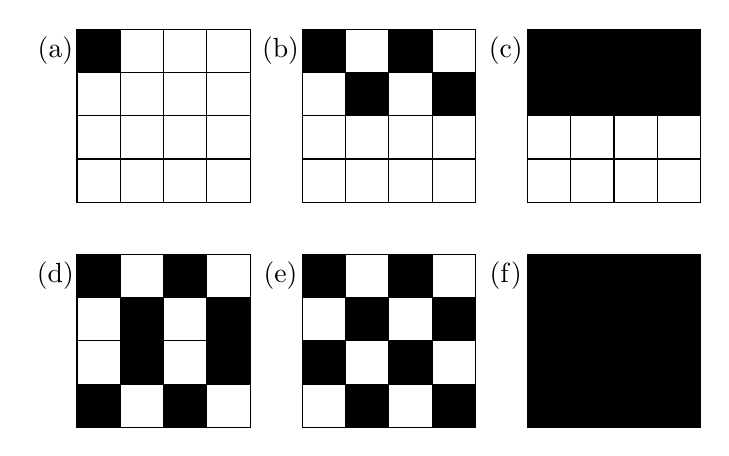
\begin{tikzpicture}[x=0.55cm, y=0.55cm] % {{{
\pgfmathsetmacro{\unitstep}{5.2}
\begin{scope}[shift={(1*\unitstep,0)}] % Depolirizng channel {{{
\node at (-0.5,0.5) {(a)} ;
    \foreach \x in {0,1,2,3} {
      \foreach \y in {0,1,2,3} {
        \begin{scope}[shift={(\x,-\y)}] 
          \draw (0,0) rectangle (1,1); 
%           \node at (0.5,0.5) {$\tau_{\y,\x}$};
         \end{scope}
%         \node at (0,-\y) (input\y) {$i_\y$};
%         \node[block] at (2,-\y) (block\y) {$f_\y$};
%         \draw[->] (input\y) -- (block\y);
%         \draw[->] (block\y.east) -- +(0.5,0);
    }
    }
\begin{scope}[shift={(0,0)}] \fill[black] (0,0) rectangle (1,1); \end{scope}
% \begin{scope}[shift={(3,-3)}] \fill[black] (0,0) rectangle (1,1); \end{scope}
% \begin{scope}[shift={(0,0)}] \fill[black] (0,0) rectangle (1,1); \end{scope}
% \begin{scope}[shift={(3,0)}] \fill[black] (0,0) rectangle (1,1); \end{scope}
\end{scope} % }}}
\begin{scope}[shift={(2*\unitstep,0)}] % Interseccion {{{
\node at (-0.5,0.5) {(b)} ;
    \foreach \x in {0,1,2,3} {
      \foreach \y in {0,1,2,3} {
        \begin{scope}[shift={(\x,-\y)}] 
          \draw (0,0) rectangle (1,1); 
%           \node at (0.5,0.5) {$\tau_{\y,\x}$};
         \end{scope}
%         \node at (0,-\y) (input\y) {$i_\y$};
%         \node[block] at (2,-\y) (block\y) {$f_\y$};
%         \draw[->] (input\y) -- (block\y);
%         \draw[->] (block\y.east) -- +(0.5,0);
    }
    }
\begin{scope}[shift={(0,0)}] \fill[black] (0,0) rectangle (1,1); \end{scope}
\begin{scope}[shift={(2,0)}] \fill[black] (0,0) rectangle (1,1); \end{scope}
\begin{scope}[shift={(1,-1)}] \fill[black] (0,0) rectangle (1,1); \end{scope}
\begin{scope}[shift={(3,-1)}] \fill[black] (0,0) rectangle (1,1); \end{scope}
% \begin{scope}[shift={(2,-3)}] \fill[black] (0,0) rectangle (1,1); \end{scope}
\end{scope} % }}}
\begin{scope}[shift={(3*\unitstep,0)}] % E4 {{{
\node at (-0.5,0.5) {(c)} ;
    \foreach \x in {0,1,2,3} {
      \foreach \y in {0,1,2,3} {
        \begin{scope}[shift={(\x,-\y)}] 
          \draw (0,0) rectangle (1,1); 
%           \node at (0.5,0.5) {$\tau_{\y,\x}$};
         \end{scope}
%         \node at (0,-\y) (input\y) {$i_\y$};
%         \node[block] at (2,-\y) (block\y) {$f_\y$};
%         \draw[->] (input\y) -- (block\y);
%         \draw[->] (block\y.east) -- +(0.5,0);
    }
    }
\begin{scope}[shift={(0,0)}] \fill[black] (0,0) rectangle (1,1); \end{scope}
\begin{scope}[shift={(1,0)}] \fill[black] (0,0) rectangle (1,1); \end{scope}
\begin{scope}[shift={(2,0)}] \fill[black] (0,0) rectangle (1,1); \end{scope}
\begin{scope}[shift={(3,0)}] \fill[black] (0,0) rectangle (1,1); \end{scope}
\begin{scope}[shift={(0,-1)}] \fill[black] (0,0) rectangle (1,1); \end{scope}
\begin{scope}[shift={(1,-1)}] \fill[black] (0,0) rectangle (1,1); \end{scope}
\begin{scope}[shift={(2,-1)}] \fill[black] (0,0) rectangle (1,1); \end{scope}
\begin{scope}[shift={(3,-1)}] \fill[black] (0,0) rectangle (1,1); \end{scope}
% \begin{scope}[shift={(2,-3)}] \fill[black] (0,0) rectangle (1,1); \end{scope}
\end{scope} % }}}
\begin{scope}[shift={(1*\unitstep,-\unitstep)}] % E7 {{{
\node at (-0.5,0.5) {(d)} ;
    \foreach \x in {0,1,2,3} {
      \foreach \y in {0,1,2,3} {
        \begin{scope}[shift={(\x,-\y)}] 
          \draw (0,0) rectangle (1,1); 
%           \node at (0.5,0.5) {$\tau_{\y,\x}$};
         \end{scope}
%         \node at (0,-\y) (input\y) {$i_\y$};
%         \node[block] at (2,-\y) (block\y) {$f_\y$};
%         \draw[->] (input\y) -- (block\y);
%         \draw[->] (block\y.east) -- +(0.5,0);
    }
    }
\begin{scope}[shift={(0,0)}] \fill[black] (0,0) rectangle (1,1); \end{scope}
\begin{scope}[shift={(2,0)}] \fill[black] (0,0) rectangle (1,1); \end{scope}
\begin{scope}[shift={(1,-1)}] \fill[black] (0,0) rectangle (1,1); \end{scope}
\begin{scope}[shift={(3,-1)}] \fill[black] (0,0) rectangle (1,1); \end{scope}
\begin{scope}[shift={(1,-2)}] \fill[black] (0,0) rectangle (1,1); \end{scope}
\begin{scope}[shift={(3,-2)}] \fill[black] (0,0) rectangle (1,1); \end{scope}
\begin{scope}[shift={(0,-3)}] \fill[black] (0,0) rectangle (1,1); \end{scope}
\begin{scope}[shift={(2,-3)}] \fill[black] (0,0) rectangle (1,1); \end{scope}
% \begin{scope}[shift={(2,-3)}] \fill[black] (0,0) rectangle (1,1); \end{scope}
\end{scope} % }}}
\begin{scope}[shift={(2*\unitstep,-\unitstep)}] % E11 {{{
\node at (-0.5,0.5) {(e)} ;
    \foreach \x in {0,1,2,3} {
      \foreach \y in {0,1,2,3} {
        \begin{scope}[shift={(\x,-\y)}] 
          \draw (0,0) rectangle (1,1); 
%           \node at (0.5,0.5) {$\tau_{\y,\x}$};
         \end{scope}
%         \node at (0,-\y) (input\y) {$i_\y$};
%         \node[block] at (2,-\y) (block\y) {$f_\y$};
%         \draw[->] (input\y) -- (block\y);
%         \draw[->] (block\y.east) -- +(0.5,0);
    }
    }
\begin{scope}[shift={(0,0)}] \fill[black] (0,0) rectangle (1,1); \end{scope}
\begin{scope}[shift={(2,0)}] \fill[black] (0,0) rectangle (1,1); \end{scope}
\begin{scope}[shift={(1,-1)}] \fill[black] (0,0) rectangle (1,1); \end{scope}
\begin{scope}[shift={(3,-1)}] \fill[black] (0,0) rectangle (1,1); \end{scope}
\begin{scope}[shift={(1,-3)}] \fill[black] (0,0) rectangle (1,1); \end{scope}
\begin{scope}[shift={(3,-3)}] \fill[black] (0,0) rectangle (1,1); \end{scope}
\begin{scope}[shift={(0,-2)}] \fill[black] (0,0) rectangle (1,1); \end{scope}
\begin{scope}[shift={(2,-2)}] \fill[black] (0,0) rectangle (1,1); \end{scope}
% \begin{scope}[shift={(2,-3)}] \fill[black] (0,0) rectangle (1,1); \end{scope}
\end{scope} % }}}
\begin{scope}[shift={(3*\unitstep,-\unitstep)}] % Identity channel {{{
\node at (-0.5,0.5) {(f)} ;
    \foreach \x in {0,1,2,3} {
      \foreach \y in {0,1,2,3} {
        \begin{scope}[shift={(\x,-\y)}] 
          \draw (0,0) rectangle (1,1); 
%           \node at (0.5,0.5) {$\tau_{\y,\x}$};
         \end{scope}
%         \node at (0,-\y) (input\y) {$i_\y$};
%         \node[block] at (2,-\y) (block\y) {$f_\y$};
%         \draw[->] (input\y) -- (block\y);
%         \draw[->] (block\y.east) -- +(0.5,0);
    }
    }
\begin{scope}[shift={(0,0)}] \fill[black] (0,0) rectangle (1,1); \end{scope}
\begin{scope}[shift={(0,-1)}] \fill[black] (0,0) rectangle (1,1); \end{scope}
\begin{scope}[shift={(0,-2)}] \fill[black] (0,0) rectangle (1,1); \end{scope}
\begin{scope}[shift={(0,-3)}] \fill[black] (0,0) rectangle (1,1); \end{scope}
\begin{scope}[shift={(1,0)}] \fill[black] (0,0) rectangle (1,1); \end{scope}
\begin{scope}[shift={(1,-1)}] \fill[black] (0,0) rectangle (1,1); \end{scope}
\begin{scope}[shift={(1,-2)}] \fill[black] (0,0) rectangle (1,1); \end{scope}
\begin{scope}[shift={(1,-3)}] \fill[black] (0,0) rectangle (1,1); \end{scope}
\begin{scope}[shift={(2,0)}] \fill[black] (0,0) rectangle (1,1); \end{scope}
\begin{scope}[shift={(2,-1)}] \fill[black] (0,0) rectangle (1,1); \end{scope}
\begin{scope}[shift={(2,-2)}] \fill[black] (0,0) rectangle (1,1); \end{scope}
\begin{scope}[shift={(2,-3)}] \fill[black] (0,0) rectangle (1,1); \end{scope}
\begin{scope}[shift={(3,0)}] \fill[black] (0,0) rectangle (1,1); \end{scope}
\begin{scope}[shift={(3,-1)}] \fill[black] (0,0) rectangle (1,1); \end{scope}
\begin{scope}[shift={(3,-2)}] \fill[black] (0,0) rectangle (1,1); \end{scope}
\begin{scope}[shift={(3,-3)}] \fill[black] (0,0) rectangle (1,1); \end{scope}
\end{scope} % }}}
\end{tikzpicture} % }}}
\end{center}
\caption{\cpnote{Mejorar el caption cuando me ponga de acuerdo con la gente}
Aca poner 6 PCEs. (f) Identidad, (a) totally depolarizing, (c, d y e) tres
generadores, (b) un canal que resulte del generador. Sobra un espacio para
ilustrar alguna otra cosa. Quiza poner otro generador para que se vea que no
hay una manera unica de generar esos bichos.}
\label{fig:examplesPCE}
\end{figure} % }}}
% Los canales tiene 2^K componente {{{
We can then see that all PCEs \janote{PCE quantum channels, PCEs me parece que refiere más a todos los PCE maps} preserve $2^K$ components. In fact, with the above 
picture, it is clearly revealed that the vector space has dimension $2N$. Moreover, 
consider any subspace and chose the maximum number of linearly independent
elements (say $K$).  Any of the  $2^K$ subsets of those elements will yield a
unique element. Moreover, since $\valpha + \valpha = \vec 0$, these are all
elements of the vector space. This means that any PCE\janote{quantum channel} will preserve $2^K$ 
components, for $K$ an integer. See \fref{fig:examplesPCE} for some examples. 
\par 

The dimension of the vector space $V$ of all multi-indices is $2N$, and we have
seen earlier that
\begin{equation}
W=\left\{
\vec\alpha:\vec\alpha\in V, \tau_{\vec\alpha}=1
\right\}
\label{eq:19}
\end{equation}
is a subspace of $V$. As such, $W$ has a given dimension $K$, which means that
$W$ has $2^K$ elements. In other words, a vector $\vec\tau$ with the property
discussed above can only have $2^K$ elements equal to 1, for a given integer
$K$. \par

\cpnote{Dejar que la raza elija uno de los dos parrafos anteriores}\janote{El primero (simón, cambié de opinión)} \par 

 % }}}
% Cuantos canales conservan $2^K$ componentes? {{{
It is natural to ask how many PCEs exist that conserve $2^K$ components. One
can calculate such number, $\sss_{N,K}$, by examining the number of different
independent subsets of vectors that spawn a given vector subspace. In appendix 
\ref{app:contar} we show that 
\begin{equation}
\sss_{N,K}=\prod_{m=0}^{K-1} \frac{2^{2N-m}-1}{2^{K-m}-1}.
\label{eq:conteo:main}
\end{equation}
%An elementary test is $N=3$ and $K=2,3$: 
%\begin{eqnarray}
%\sss_{3,2}&=&\frac{(2^6-1)(2^5-1)}{(2^2-1)(2^1-1)}=\frac{63\cdot31}{3}=651,\\
%\sss_{3,3}&=&\frac{(2^6-1)(2^5-1)(2^4-1)}{(2^3-1)(2^2-1)(2^1-1)}=\frac{63\cdot31\cdot15}{7\cdot3}=1395,
%\end{eqnarray}
%which are indeed the values found numerically. 
From the above expression, it is easy to see the symmetry relation
\begin{equation}\label{eq:conteo:simmetry}
\sss_{N,K}=\sss_{N,2N-K}
\end{equation}
which suggest an\janote{a*} relation  between individual channels\janote{that
preserve $K$ and $2N-K$ Pauli components} that for the time being
has escaped our efforts to identify. 
\par % }}}
% Frase de David {{{
\ddnote{Agrego esto:} A final remarks of the derivation as a tool. Concepts
might be complicated, but the tool gives some simple rules to the reader:
\textit{tell me what components you want to keep, and the (vector) summation
rules will give you the rest of components to make the target operation a CPTP
one.} \janote{Me gusta esto que puso David, pero lo movería a las conclusiones.}
\par % }}}

% }}}


